\documentclass[aspectratio=43]{beamer}%[handout]
\mode<handout>{
\usepackage{pgfpages}
\pgfpagesuselayout{4 on 1}[letterpaper,border shrink=5mm, landscape]
}
\usepackage[T1]{fontenc}
\usepackage[utf8]{inputenc}
\usepackage[spanish]{babel}
\usepackage{beamerthemeshadow,beamerthemesplit,cite,cancel,lmodern,eso-pic,fancyvrb,textcomp,lmodern,url,times,booktabs,amssymb,amsmath,ragged2e,float,subfig,xspace,epic,eepic,multicol,multirow,colortbl,color,graphicx,url}
\usepackage[normalem]{ulem} %tachar texto con \sout{}
\usepackage{listings} %CODIGOs
\usepackage[sfdefault]{roboto}
\setcounter{tocdepth}{3}
\usepackage[figurename=]{caption}
%Colores Ulagos
\definecolor{gray97}{gray}{.97}
\definecolor{gray75}{gray}{.75}
\definecolor{gray45}{gray}{.45}
\definecolor{listinggray}{gray}{0.9}
\definecolor{lbcolor}{rgb}{0.9,0.9,0.9}
%Colores Ulagos
\definecolor{amarillo}{RGB}{255,182,18}
\definecolor{verde}{RGB}{52,178,51}
\definecolor{rojo}{RGB}{237,41,57}
\definecolor{azulu}{RGB}{19,15,204}
\definecolor{azul}{RGB}{1,110,185}
\definecolor{negro}{RGB}{35,31,32}
\definecolor{naranjo}{RGB}{251,79,20}
\newcommand\rojo[1]{\textcolor[RGB]{237,41,57}{#1}}
\newcommand\gris[1]{\textcolor[gray]{.65}{#1}}
\newcommand\azul[1]{\textcolor[RGB]{19,15,204}{#1}}
\newcommand\verde[1]{\textcolor[RGB]{5,101,99}{#1}}
\newcommand\naranjo[1]{\textcolor[RGB]{251,79,20}{#1}}

%%%%%%%%%%%%%%%%%%%%%%%%%
%% Tikz
%%%%%%%%%%%%%%%%%%%%%%%%%
\usepackage{tikz}
\usetikzlibrary{trees}
\usetikzlibrary{snakes}
\usetikzlibrary{arrows}
\usetikzlibrary{shapes}
\usetikzlibrary{backgrounds}
\usetikzlibrary{patterns}
\usetikzlibrary{fit}
\usetikzlibrary{positioning} % LATEX and plain TEX
%%%%%%%%%%%%%%%%%%%%%%%%%%

%%%%%%%%%%%%%%%%%%%%%TEMA
\mode<presentation>
\usetheme{CambridgeUS}
\usecolortheme[named=azul]{structure}
\useinnertheme{rectangles}    
\useoutertheme{infolines} 
               
\setbeamercovered{transparent}

\setbeamerfont{block title}{size={}}
\setbeamerfont{title}{shape=\scshape}
\setbeamerfont{frametitle}{shape=\scshape}
\setbeamerfont{author}{shape=\scshape}
\setbeamerfont{institute}{shape=\scshape}
\setbeamerfont{block title}{shape=\scshape}

\setbeamertemplate{blocks}[rounded][shadow=true]
\setbeamertemplate{itemize items}[default]
\setbeamertemplate{enumerate items}[circle]
\setbeamertemplate{description item}[align left]
\setbeamertemplate{blocks}[rounded][shadow=true]
\setbeamertemplate{title page}[default][colsep=-4bp,rounded=false,shadow=false]
%\setbeamertemplate{frametitle continuation}

\setbeamercolor*{palette primary}{use=structure,fg=azul,bg=listinggray}
\setbeamercolor*{palette secondary}{use=structure,fg=azul,bg=gray97}
\setbeamercolor*{palette tertiary}{use=structure,fg=gray97,bg=azul}
\setbeamercolor*{palette sidebar primary}{use=structure,fg=azul}
\setbeamercolor*{palette sidebar tertiary}{use=structure,fg=azul}
\setbeamercolor*{title}{use=structure,fg=white}
\setbeamercolor*{author}{use=structure,fg=white}
\setbeamercolor*{institute}{use=structure,fg=white}
\setbeamercolor{frametitle right}{bg=azul!50!white}
\setbeamercolor{structure}{fg=azul}
\setbeamercolor{block title}{use=structure,fg=white,bg=amarillo}
\setbeamercolor{block body}{use=structure,fg=negro,bg=amarillo!20!white}
\setbeamercolor{block title example}{use=structure,fg=white,bg=verde!80!black}
\setbeamercolor{block body example}{use=structure,fg=negro,bg=verde!20!white}
\setbeamercolor{block title alerted}{use=structure,fg=white,bg=rojo!90!negro}
\setbeamercolor{block body alerted}{use=structure,fg=negro,bg=rojo!20!white}
%%%%%%%%%%%%%%%%%%%%%FIN TEMA

%lstlisting %%%%%CODIGOS
\lstset{tabsize=4,language=C,basicstyle=\small,upquote=true,aboveskip={1.5\baselineskip},columns=fixed,showstringspaces=false, extendedchars=true,breaklines=true, prebreak = \raisebox{0ex}[0ex][0ex]{\color{gray75}{\ensuremath{\hookleftarrow}}},showtabs=false,showspaces=false,showstringspaces=false,identifierstyle=\ttfamily,keywordstyle=\color[rgb]{0,0,1}, commentstyle=\color[rgb]{0.133,0.545,0.133}, stringstyle=\color[rgb]{0.627,0.126,0.941}} 
  
%%%%%%%%%%%%%%PORTADA
\title[Bibliografía en \LaTeX{}]{\textbf{\huge{Bibliografía en \LaTeX{}}}\vspace{-0.3cm}}
%\subtitle{subtitulo\vspace{-0.7cm}}
\author[Juan José Ramírez Lama]{\small{\textbf{Juan José Ramírez Lama} \\ \texttt{juan.ramirez@ulagos.cl} }\vspace{-0.2cm}}
\institute[ULA]{\small{\textbf{Departamento de Ciencias Exactas}\\Ingeniería Civil en Informática}\vspace{-0.5cm}}
\date[\today]{}
%%%%%%%%%%%%%FIN PORTADA

\begin{document}
\setbeamertemplate{background}{
\includegraphics[height=9.2cm,width=12.8cm]{fondoula43}}%4:3
%\setbeamertemplate{background}{\centering\includegraphics[height=8.6cm,width=16.1cm]{fondoula169}}%16:9


%Pagina de Portada
\begin {frame} [plain]
\vspace{5.25cm}
\titlepage
\end {frame}
\setbeamertemplate{background}{}
%%%%%%%%%%%%%%%%ÍNDICES
\section[Contenido]{}
\frame{
  \frametitle{\textbf{Contenido}}
\setcounter{tocdepth}{2}%1: solo titulo principal, 2: titulo y subtitulo, 3....
\scriptsize
\tableofcontents[]
}%Generacion de Indice por capitulo
\AtBeginSection[]{
\begin{frame}
\frametitle{\textbf{Contenido}}
\scriptsize
\tableofcontents[currentsection]
\end{frame}}

\AtBeginSubsection[]{
\begin{frame}
\frametitle{\textbf{Contenido}}  
\scriptsize
\tableofcontents[currentsection,currentsubsection]
\end{frame}
}
%%%%%%%%%%%%%%%%FIN ÍNDICES







%%%%%%%%%%%%%%%%%%%%%%%%%%%%%%%%%%%%%
%%%%%%%%%%%%%%%%%INICIO PRESENTACION
\section{Introducción}
\subsection{Bibliografía en \LaTeX{}}
\begin{frame}[fragile]
\frametitle{\textbf{Bibliografía en \LaTeX{}}}
\justifying
 \begin{itemize}\justifying
  \item Gestión de bibliografía: Muy importante en el mundo académico y de investigación.
  \item \LaTeX{} dispone de un sistema básico de gestión de bibliografía integrado.
  \item Bib\TeX{} es un paquete incluido en la instalación por defecto de \LaTeX{} que permite gestionar la bibliografía de formas más avanzadas.
\end{itemize}

\end{frame}

\subsection{Características de Bib\TeX{}}
\begin{frame}[fragile]
\frametitle{\textbf{Características de Bib\TeX{}}}
\justifying
 \begin{itemize}\justifying
  \item Independencia del documento: bibliografía almacenada en archivos externos de texto plano.
  \item Uniformidad del formato: Bib\TeX{} define en qué formato se definen las referencias, en función de estilos que le hayamos indicado.
  \item Organización: Se pueden tener varios archivos de bibliografía, separando así las referencias por temas.
\end{itemize}
\end{frame}


\section{Bibliografía Integrada}
\subsection{Características}
\begin{frame}[fragile]
\frametitle{\textbf{Características}}
\justifying
 \begin{itemize}\justifying
  \item Útil cuando no se espera reutilizar la bibliografía.
  \begin{itemize}\justifying
  \item[] Ejemplo: si se escribe un documento sobre un tema que no se trata con frecuencia.
\end{itemize}

  \item Entorno \texttt{thebibliography}. Se pone donde se quiera insertar la bibliografía (normalmente justo al final del documento).
  \item A diferencia de Bib\TeX{}, nosotros indicamos el formato de cada elemento. Puede no ser un formato uniforme.
\end{itemize}

\end{frame}

\subsection{Formato}
\begin{frame}[fragile]
\frametitle{\textbf{Formato}}
\justifying
 \begin{itemize}\justifying
  \item Dentro del entorno se escriben los datos bibliográficos.
  \item Formato: \texttt{$\textbackslash$bibithem\{label\}} datos bibliográficos, más datos, últimos datos.
  \item La etiqueta (label) es algo interno, para facilitarnos identificar la referencia. No se mostrará en ninguna parte.
  \item Como etiqueta (label) se puede usar el apellido del autor, dos dígitos del año de la publicación, y si hay varias publicaciones ese año, una letra, etc.
  \item Después de la etiqueta se ponen datos como el autor, el título, etc.
  \item Se suele separar en varias líneas por legibilidad.
\end{itemize}

\end{frame}

\subsubsection{Ejemplo}
\begin{frame}[fragile]
\frametitle{\textbf{Ejemplo}}
\justifying
 \begin{exampleblock}{}
   \vspace{-0.7cm}
\begin{lstlisting}
\begin{thebibliography}{99}
\bibitem{lamport94}
Leslie Lamport, \emph{\LaTeX : A Document Preparation System}. Addison Wesley, Massachusetts, 2nd Edition, 1994.
\end{thebibliography}
\end{lstlisting}\vspace{-0.3cm}

\end{exampleblock}

\begin{block}{}
\begin{thebibliography}{99}
\bibitem{lamport94} Leslie Lamport, \emph{\LaTeX : A Document Preparation System}. Addison Wesley, Massachusetts, 2nd Edition, 1994.
\end{thebibliography}
\end{block}


\end{frame}

\subsection{Formato APA}
\begin{frame}[fragile]
\frametitle{\textbf{Formato APA}}
\justifying
 El formato para escribir la bibliografía en formato APA es la siguiente:
\begin{block}{sintaxis}
   \lstset{language=}%SQL,basicstyle=\small}
   \vspace{-0.8cm}
\begin{lstlisting}
\bibitem [Apellidos, Año]{Referencia} Apellidos, Nombres (Año). Titulo, Revista, Edición, Paginas.
\end{lstlisting}\vspace{-0.3cm}

\end{block}
Entre los corchetes van los datos que deseamos que aparezca en la cita.
\end{frame}

\begin{frame}[fragile]
\frametitle{\textbf{Ejemplo}}
\justifying
 \begin{exampleblock}{Código}
   \vspace{-0.8cm}
\begin{lstlisting}
\begin{thebibliography}{99}
\bibitem [Gutierrez, 2003]{001} Gutierrez, R. M. (2013). El impacto de la sobrepoblación de invertebrados en un ecosistema selvático . Revista Mundo Natural, 8, 73-82.
\end{thebibliography}  
\end{lstlisting}\vspace{-0.3cm}
\end{exampleblock}

\begin{block}{Resultado}
\begin{thebibliography}{99}
\bibitem [Gutierrez, 2003]{001} Gutierrez, R. M. (2013). El impacto de la sobrepoblación de invertebrados en un ecosistema selvático . Revista Mundo Natural, 8, 73-82.
\end{thebibliography}
\end{block}


\end{frame}


\subsection{Citando las Referencias}
\begin{frame}[fragile]
\frametitle{\textbf{Citando las Referencias}}
\justifying
 Las referencias no se insertan directamente en la bibliografía: hay que citarlas.
 \begin{description}\justifying
  \item[\texttt{$\textbackslash$cite\{label\}}] cita una referencia, de forma que aparecerá en la bibliografía.
  \begin{itemize}\justifying
  \item Se puede citar una página concreta del documento:\\\texttt{$\textbackslash$cite[p. 215]\{lamport94\}}.
  \item Se pueden citar varias referencias a la vez:\\ \texttt{$\textbackslash$cite\{lamport94, rodriguez05, torres09\}}.
\end{itemize}
\item [\texttt{$\textbackslash$nocite\{label\}}] Permite incluir una referencia sin que se haya citado en el texto.
\item [\texttt{$\textbackslash$nocite\{*\}}] Incluye todas las referencias.
\end{description}

\end{frame}


\begin{frame}[fragile]
\frametitle{\textbf{Cita en formato APA}}
\justifying
 \begin{exampleblock}{Citando}
   \vspace{-0.8cm}
\begin{lstlisting}
Aquí se esta haciendo mención al articulo de \cite{001} que es en Formato APA y al de \cite{lamport94} que está en formato genérico.
\end{lstlisting}\vspace{-0.3cm}
\end{exampleblock}


\end{frame}


\section{Bib\TeX{}}
\subsection{Introducción}
\begin{frame}[fragile]
\frametitle{\textbf{Gestión de Bibliografía con Bib\TeX{}}}
\justifying
 Caracteristicas:
 \begin{itemize}\justifying
  \item Permite gestión bibliográfica más avanzada.
  \item Muy recomendable para reutilizar bibliografía.
  \item Muy flexible.
  \item La bibliografía se almacena en un archivo de texto plano \texttt{.bib}.
  \item Requiere compilar con \texttt{bibtex} para que detecte la bibliografía.
\end{itemize}

\end{frame}

\begin{frame}[fragile]
\frametitle{\textbf{Gestión de Bibliografía con Bib\TeX{}}}
\justifying
 \begin{block}{}\small
   \vspace{-0.7cm}
\begin{lstlisting}
@tipoentrada{label , 
campo1 = "Valor campo 1", 
campo2 = "Valor Campo 2",
campo3 = "Valor Campo 3",
[...]
campon = " Valor Campo n ",
}
\end{lstlisting}\vspace{-0.3cm}

\end{block}

\begin{exampleblock}{}\small
\begin{verbatim}
@article{greenwade 93,
author = "George D . Greenwade", 
title = "The {C}omprehensive {T}ex {A}rchive {N}etwork
 ({CTAN})", 
year = "1993",
journal = "TUGBoat", 
volume = "14", 
number = "3",
pages = "342−−351"}
\end{verbatim}

\end{exampleblock}


\end{frame}

\subsection{Formato de las Entradas}


\begin{frame}[fragile]
\frametitle{\textbf{Formato de las Entradas}}
\justifying
 \begin{itemize}\justifying
  \item Los campos de cada entrada dependen del tipo de entrada.
\pause  \item \textbf{Tipos de entradas}\footnote{\url{http://newton.ex.ac.uk/tex/pack/bibtex/btxdoc/node6.html}}:\texttt{required}, \texttt{optional}, \texttt{ignored}, \texttt{article}, \texttt{book}, \texttt{booklet}, \texttt{conference}, \texttt{inbook}, \texttt{incollection},  \texttt{misc}, \texttt{inproceedings},   \texttt{mastersthesis}, \texttt{phdthesis}, \texttt{proceedings}, \texttt{techreport}, \texttt{unpublished}, \texttt{manual}.
 \pause \item \textbf{Campos}\footnote{\url{http://newton.ex.ac.uk/tex/pack/bibtex/btxdoc/node7.html}}: \texttt{address}, \texttt{annote}, \texttt{author}, \texttt{booktitle}, \texttt{chapter}, \texttt{crossref}, \texttt{edition}, \texttt{editor}, \texttt{howpublished}, \texttt{institution}, \texttt{journal}, \texttt{key}, \texttt{month}, \texttt{note}, \texttt{number}, \texttt{organization}, \texttt{pages}, \texttt{publisher}, \texttt{school}, \texttt{series}, \texttt{title}, \texttt{type}, \texttt{volume}, \texttt{year}.
\pause  \item Para mantener las mayúsculas y minúsculas, encerrar el texto entre llaves.
\end{itemize}

\scriptsize
\begin{verbatim}
title = "The {C}omprehensive {T}ex {A}rchive {N}etwork ({CTAN})", 
\end{verbatim}
\end{frame}



\begin{frame}[fragile]
\frametitle{\textbf{Formato de las Entradas}}
\justifying
 \begin{exampleblock}{}
   \vspace{-0.7cm}
\begin{lstlisting}
@article{AbedonHymanThomas 2003,
author = "Abedon, S. T. and Hyman, P. and Thomas, C.",
year = "2003",
title = "Experimental examination of bacteriophage latent-
period evolution as a response to bacterial availability",
journal = "Applied and Environmental Microbiology", volume = "69",
pages = "7499−−7506"
}
\end{lstlisting}\vspace{-0.3cm}
\end{exampleblock}
\end{frame}

\begin{frame}[fragile]
\frametitle{\textbf{Formato de las Entradas}}
\justifying
 \begin{exampleblock}{}
   \vspace{-0.7cm}
\begin{lstlisting}
@MISC{website : fermentas−lambda,
AUTHOR = "Fermentas Inc.",
TITLE = "Phage Lambda: description \& restriction map", MONTH = "November",
YEAR = 2008,
HOWPUBLISHED = "\url{http://www.fermentas.com/techinfo/nucleicacids/maplambda.htm}"}
\end{lstlisting}\vspace{-0.3cm}
\end{exampleblock}
\end{frame}


\subsection{Inclusión de la Bibliografía}
\begin{frame}[fragile]
\frametitle{\textbf{Inclusión de la Bibliografía}}
\justifying
 Comandos para inclusión de bibliografía.
 \begin{itemize}\justifying
  \item \texttt{$\textbackslash$bibliographystyle\{formato\}}
  \item \texttt{$\textbackslash$bibliography\{archivo1, archivo2, archivo3\}}
\end{itemize}
\pause Citar Referencias:
\begin{itemize}\justifying
  \item \texttt{$\textbackslash$cite\{label\}}, \texttt{$\textbackslash$nocite\{label\}}, \texttt{$\textbackslash$nocite\{*\}}.
\end{itemize}
\pause Formatos de Bibliografía:
\begin{itemize}\justifying
  \item Se seleccionan con \texttt{$\textbackslash$bibliographystyle\{formato\}}.
\begin{description}\justifying
  \item [formato]\texttt{plain}, \texttt{abbrv}, \texttt{alpha}, \texttt{ieeetr}, \texttt{apacite}.
\end{description}
El formato \texttt{apacite} requiere el paquete \texttt{apacite}.

\end{itemize}
\end{frame}



\subsection{Estilos de Bibliografía}
\begin{frame}[fragile]
\frametitle{\textbf{plain}}
\justifying
 \begin{center}
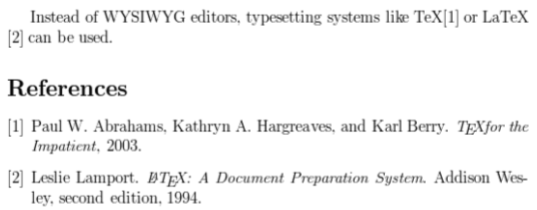
\includegraphics[width=12cm]{images/plain}
\end{center}

\end{frame}

 \begin{frame}[fragile]
\frametitle{\textbf{abbrv}}
\justifying
 Muestra los nombres de los autores abreviados.
 
 \begin{center}
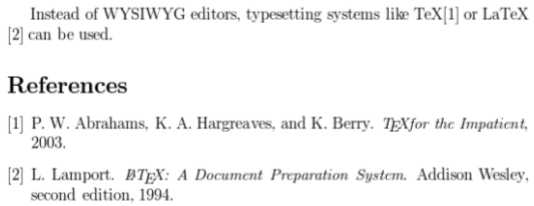
\includegraphics[width=12cm]{images/abbrv}
\end{center}

\end{frame}



\begin{frame}[fragile]
\frametitle{\textbf{alpha}}
\justifying
 Muestra las referencias identificadas con letras en lugar de numéricamente.
 
 \begin{center}
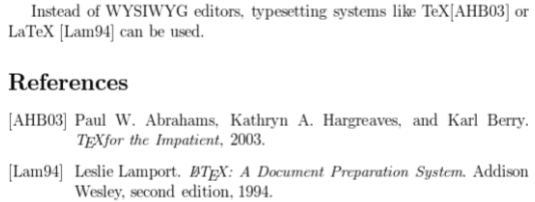
\includegraphics[width=12cm]{images/alpha}
\end{center}

\end{frame}

\begin{frame}[fragile]
\frametitle{\textbf{ieeetr}}
\justifying
 Ordena las referencias por orden de aparición en lugar de orden alfabético.
 
 \begin{center}
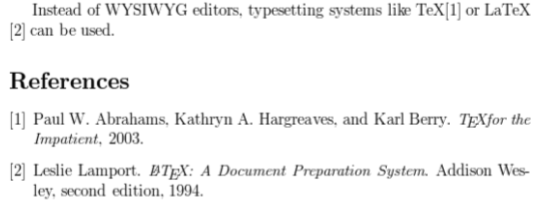
\includegraphics[width=12cm]{images/ieeetr}
\end{center}

\end{frame}

\begin{frame}[fragile]
\frametitle{\textbf{apacite}}
\justifying
 Es el formato APA, ordena las referencias por orden alfabetico de apellido.
 
 \begin{center}

\includegraphics[width=10cm]{images/apacite}\\
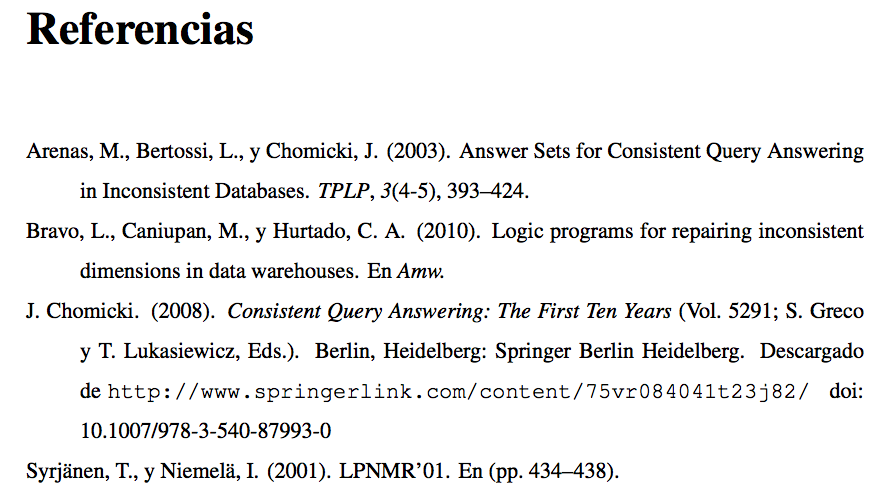
\includegraphics[width=9cm]{images/aparef}
\end{center}

 
\end{frame}




\begin{frame}[fragile]
\frametitle{\textbf{Otros estilos de Bibliografía}}
\justifying
 \begin{itemize}\justifying
  \item Muchas publicaciones tienen estilos de bibliografía propios.
  \item Por ejemplo, si escribimos un artículo científico para una revista.
  \item Muchas publicaciones tienen estilos de bibliografía propios.
  \begin{itemize}\justifying
  \item Por ejemplo, si escribimos un artículo científico para una revista.
  \item En este caso, nos proporcionarán un archivo \texttt{.bst}, y podremos usar ese estilo en lugar de los que vienen por defecto.
  \item [] Ejemplo: si el archivo es \texttt{h-physrev3.bst}, en el documento tendremos que escribir \texttt{$\textbackslash$bibliographystyle\{h-physrev3.bst\}}.
\end{itemize}
\begin{block}{Administrador de Bibliografía}
Existen varios administradores de Bibliografía: \textbf{Mendeley} y \textbf{Zotero} son algunos de ellos.
\begin{itemize}\justifying
  \item Al exportar las bibliografías, revisa las etiquetas que se han asignado. Es recomendable cambiarlas por otras que se recuerden más fácilmente.
  \item Si hay caracteres no válidos en las etiquetas, hay que eliminarlos.
\end{itemize}
\end{block}
\end{itemize}
\end{frame}


\section{Ejemplo}
\begin{frame}[fragile]
\frametitle{\textbf{Ejemplo archivo bibliografia.bib}}
\justifying
 \begin{block}{}
   \vspace{-0.7cm}
      \lstset{basicstyle=\scriptsize}

\begin{lstlisting}
@misc{Nobody 06, author = "Nobody Jr" , title = "My Article" , year = "2006"}
@InProceedings{irusta_sequential_2007,
title = "Sequential {VT/VF} discrimination algorithm based on wave mode sample entropy for adult and pediatric patients" , isbn = "0276−6547",
url = "10.1109/CIC.2007.4745463",
doi = "10.1109/CIC.2007.4745463",
abstract = "The two fatal ventricular arrhythmias, Ventricular Fibrillation {(VF)} and Ventricular Tachycardia {(VT),} are better treated using different electrical therapies: a lower energy cardioversion for {VT} and a defibrillation shock for {VF.}"
author = "U. Irusta and J. Ruiz and {S.R.} de Gauna and E. Aramendi",
year = "2007",
keywords = "adult patients , automated external defibrillators, defibrillation shock, {ECG,}", pages = "229−−232"
}
\end{lstlisting}\vspace{-0.3cm}
\end{block}
\end{frame}



\begin{frame}[fragile]
\frametitle{\textbf{Archivo documento.tex}}
\justifying
 \begin{block}{}
   \vspace{-0.7cm}
\begin{lstlisting}
\documentclass[10pt, letter]{article}
\usepackage[utf8]{inputenc}
\begin{document}
El documento "Sequential {VT/VF} discrimination algorithm..." \cite{irusta_sequential_2007} profundiza en este tema. % Generamos la bibliografia
\bibliographystyle{plain} 
\bibliography{bibliografia}
\end{document}
\end{lstlisting}\vspace{-0.3cm}

\end{block}

\end{frame}


\end{document}